% Question  ##################################################################################################################
\section{Question 1}\label{ssec:pt1q1}
\textbf{The objective of this question is to analyse the data for different instruments, based on last year’s data, and provide your opinion in terms of their respective risk and return.}

% END Question  ##############################################################################################################

% Question (i) ###############################################################################################################

\subsection{Q1 (i)}\label{sssec:pt1q1i}
\textbf{Download daily closing price data for S\&P500, FTSE100 and Gold (SPDR) for the years 2014 to 2017.}

\noindent
Code to download the closing prices for the assets specified in this question can be found in ‘Question 1 (i)’ in the python notebook. The data was downloaded from Yahoo Finance and saved as .csv format in the following path \textit{‘src/data/part\_1’}. The files were saved as follows \textit{‘FTSE100.csv’}, \textit{‘S\&P500.csv’} and \textit{‘GOLD.csv’}. The data was then reloaded from the files and converted into pandas dataframes. 

% END Question (i) ###########################################################################################################

% Question (ii) ##############################################################################################################

\subsection{Q1 (ii)}\label{sssec:pt1q1ii}
\textbf{Why log returns are normally preferred from standard arithmetic returns?}

\noindent
Log returns are preferred over arithmetic returns for several reasons, one of which is that when using log returns you are inherently normalizing all the values. The process of normalization makes the returns easier to compare with and this is very useful in analytical situations or machine learning. Another advantage is time-additivity, meaning when using log-returns it is easier to compound returns since you only need to add the values unlike when using arithmetic returns \cite{meucci2010quant}. Also, in theory prices are assumed to be distributed log normally (not always true for every price series) and transforming to log makes the values normally distributed. This is very useful in situations where it is assumed that the values are normally distributed, which is quite common in machine learning and statistics.

% END Question (ii) ##########################################################################################################

% Question (iii) #############################################################################################################

\subsection{Q1 (iii)}\label{sssec:pt1q1iii}

\textbf{Identify the first 4 distribution moments for each index/product mentioned in part (i). For your
calculations utilise daily log returns. In your answer describe the calculations/steps performed.}

\noindent
First the log returns were calculated for each index/product using the adjusted closing price. Once the log returns were computed a new column was added in each pandas dataframe called “Log Returns”, so it can be utilised when calculating the distribution moments.  A function to compute the log returns was created in the ‘fintech’ library and another function was also created to compute the four distribution moments. These functions can be shown in Fig.~\ref{fig:logretfunc} and Fig.~\ref{fig:distmomfunc}. The first and second distribution moments were calculated using numpy \cite{python:numpy} functions. The third and the forth distribution moments were calculated using scipy \cite{python:scipy}. \\

\begin{figure}[H]
\centering
  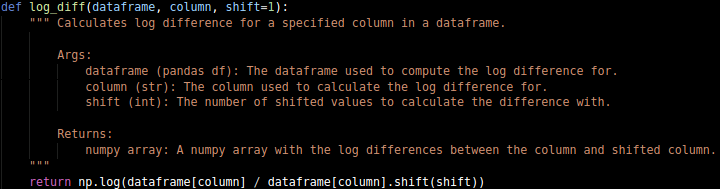
\includegraphics[scale = .65]{imgs/log_diff_func.png}
  \caption{Function to compute log returns.}
  \label{fig:logretfunc}
\end{figure}

\begin{figure}[H]
\centering
  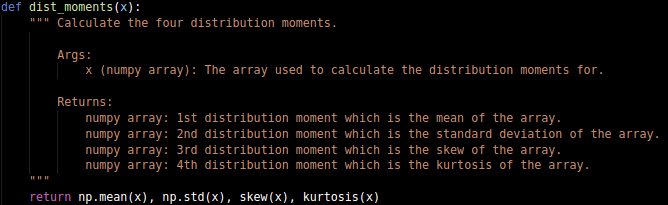
\includegraphics[scale = .7]{imgs/dist_mom_func.png}
  \caption{Function to compute four distribution moments.}
  \label{fig:distmomfunc}
\end{figure} \\

\noindent
To further explain these functions used in the code, the following equations are presented. Eq.~\ref{eq:logdiff} is used to compute the log returns, which basically takes the natural log of the adjusted price at $t$ divided by the adjusted price at $t - 1$.

\begin{equation} \label{eq:logdiff}
    Log \ Returns = \ln(\frac{S_t}{S_{t-1}})
\end{equation}

\noindent
The first distribution moment is calculated using the Eq.~\ref{eq:1mom} which basically is the mean of the computed log returns. By finding the mean of the log returns we get a value of the expected return and it gives us the centre point under the distribution. The second distribution moment as shown in Eq.~\ref{eq:2mom} is the standard deviation of the log returns. Such value shows us the volatility of the index/product and measures the disperation in the distribution.

\noindent
The third moment is the computed Skew of the log returns and this is shown in Eq.~\ref{eq:3mom}. Skew is calculated by taking the sum of the log return $Y_i$ subtracted by the log return mean $\overline{Y}$ and raised to the power of 3. Then this summation is divided by the number of the log return values ($N$). After doing so this result is divided by the standard deviation raised to the power of 3  which is shown as $s^3$. This gives us the measure of symmetry for the distribution and show us how skewed the log returns are. Similarly the fourth moment, which is also know as Kurtosis, is calculated in the same way but raised to the power of 4 as shown in Eq.~\ref{eq:4mom}. This measures the shape of our distribution for the log returns (tails, tall or flat) and the distribution is set to be normally distributed if it is close to 3. 

\begin{equation} \label{eq:1mom}
    1st \ Moment = \frac{\Sigma x}{N}
\end{equation}

\begin{equation} \label{eq:2mom}
    2nd \ Moment = \sqrt{\frac{\Sigma(x - \overline{x})^2}{N}}
\end{equation}

\begin{equation} \label{eq:3mom}
    3rd \ Moment = \frac{\sum_{i=1}^{N}(Y_i - \overline{Y})^3 / N}{s^3}
\end{equation}

\begin{equation} \label{eq:4mom}
    4th \ Moment = \frac{\sum_{i=1}^{N}(Y_i - \overline{Y})^4 / N}{s^4}
\end{equation}

\noindent
The functions described above were called from the notebook as shown in Fig.~\ref{fig:momcode} and the other Fig.~\ref{fig:momresults} shows the output of the distribution moments for each index/product. 

\begin{figure}[H]
\centering
  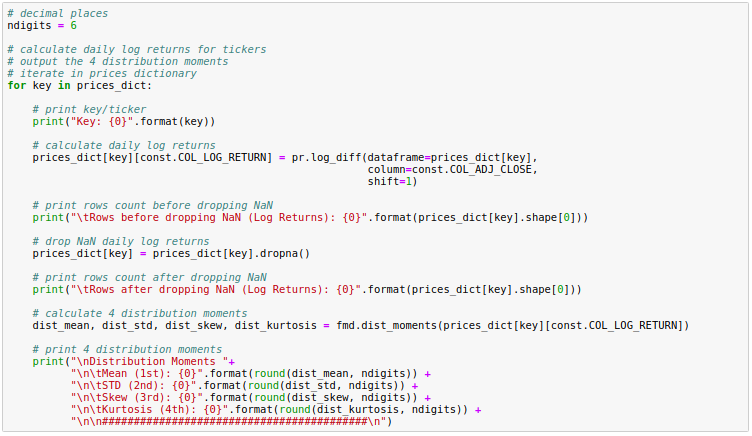
\includegraphics[scale = .60]{imgs/moments_code.png}
  \caption{Code used in the notebook to get distribution moments.}
  \label{fig:momcode}
\end{figure}

\begin{figure}[H]
\centering
  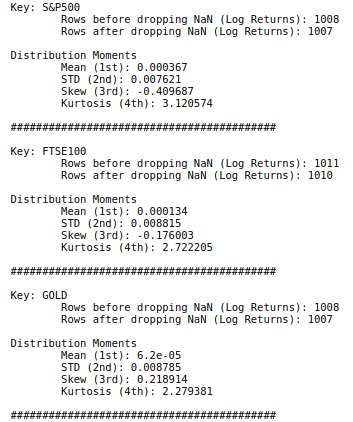
\includegraphics[scale = .60]{imgs/moments_results.png}
  \caption{Function to compute log returns }
  \label{fig:momresults}
\end{figure}

% END Question (iii) #########################################################################################################

% Question (iv) ##############################################################################################################

\subsection{Q1 (iv)}\label{sssec:pt1q1iv}

\textbf{Comment on the measured statistics from the perspective of risk and return. In your answer
compare the results obtained.}

\noindent
As described the first moment is the expected return of an asset, while the second moment gives as the expected volatility of an asset. This means that the volatility gives as the dispersion of where the price might go. The higher the volatility the larger the swings for the price over time, which can make an asset quite risky since the price can move in an upward or downward direction. The Skew measure will help us determine the extremes of where the price might go. The more skewed an asset is the less accurate financial models will be, since most of them rely on normally distributed data. When having a positively skewed returns, means that there were frequent small losses and a few large gains, while a negatively skewed returns, means that there were frequent small gains and a few large loses. In terms of risk and reward an attractive asset would be an asset with the following traits; high expected returns, low volatility, a positive skew and a Kurtosis measure close to 3 (normal distribution). 

\noindent
Looking at the S\&P500 statistics the expected returns (0.036\%) and volatility (0.7621\%) is more attractive in terms of risk and return than the FTSE100 index with expected returns (0.0134\%) and volatility (0.8815\%). This is because S\&P500 has higher expected return with less volatility making it a safer bet according to historic data. Both assets have a negative Skew and the Kurtosis measure for both assets are close to 3 with a difference of +0.120574 and –0.2278 respectively.

\noindent
On the other hand, the gold asset has an expected return (0.0062\%) and volatility (0.8785\%), which although it is less volatile than the FTSE100, the expected return is significantly lower. Unlike the other assets, the FTSE100 has a positively skewed return which is preferred over negatively skewed values. Also, the Kurtosis is close to 3 with a difference of -0.72061. 

\noindent
In terms of risk and return, the most attractive asset from the results obtained is the S\&P500 index. 

% END Question (iv) ##########################################################################################################

% Question (v) ###############################################################################################################

\subsection{Q1 (v)}\label{sssec:pt1q1v}

\textbf{Annualize daily return (first moment) and volatility (second moment). In your scaling process assume 250 days for the year. In your answer describe the calculations/steps performed.}

\noindent
The code for this task can be found in ‘Question 1 (v)’ in the python notebook. A function called ‘annretvol\_asset’ was created in the ‘fintech’ library to annualize the log returns and volatility. This function is shown in Fig.~\ref{fig:annasset}.  

\begin{figure}[H]
\centering
  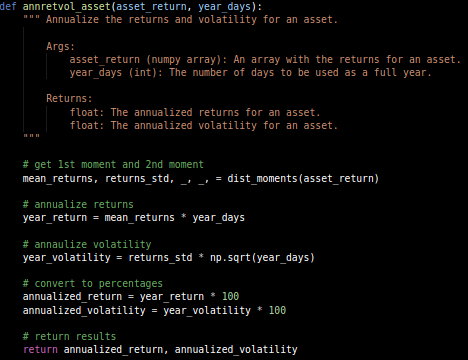
\includegraphics[scale = .65]{imgs/annualize_asset.png}
  \caption{Function to annualize returns and volatility for an asset. }
  \label{fig:annasset}
\end{figure}

\noindent
In the first line of the function the first moment and second moment are computed for the specific asset. Once these are computed the daily log return is annualized by simply using ($First \ moment \times 250$) and the volatility is annualized using  ($Second \ moment \times \sqrt{250}$). The formulas described were used since returns scale with time, while volatility scales with square root of time. The computed values are then converted to percentages and returned by the function. To calculate the annualized returns and volatility for each asset, this function was called from a loop and the daily log returns found in (iii) were passed as a parameter. Results for these two measurements are shown in Fig.~\ref{fig:annassetresult}. 

\begin{figure}[H]
\centering
  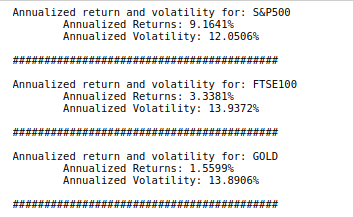
\includegraphics[scale = .75]{imgs/annualize_asset_results.png}
  \caption{Annualized returns and volatility for the three assets. }
  \label{fig:annassetresult}
\end{figure}

% END Question (v) ###########################################################################################################

% Question (vi) ##############################################################################################################

\subsection{Q1 (vi)}\label{sssec:pt1q1vi}

\textbf{By considering the last closing price at the end of 2017, and the annualized volatility from question (v), what would be the price level of S&P 500 after 1 month, that according to normal probability, there is a 32\% chance that the actual price will be above it. Show your workings.}

\noindent
Code for this task can be found in ‘Question 1 (vi)’ in the python notebook. To find the price level for the asset after one month the last closing price was fetched, which was equal to \$2,673.61. After doing so the annualized volatility $(12.05\%)$ was scaled to one month using the following formula $(\frac{12.05}{100} \times \sqrt{\frac{20}{250}})$ and it was assumed that a one month period contains 20 days. Using these two values the price deviation could be computed using $(\$2,673.61 \times (\frac{12.05}{100} \times \sqrt{\frac{20}{250}}))$ which outputs \$91.12. So the price levels after one month is in the range of ($\$2,673.61 - \$91.12$) to ($\$2,673.61 + \$91.12$) which is equal to the range of \$2,582.49 - \$2,764.73.

\noindent
Using the Z-score equation as shown in Eq.~\ref{eq:zscore}, we can find the number of standard deviations a value is from the mean. In this case the mean is set to be the last closing price for the asset, which is equal to \$2,673.61. We found that the price has a 16\% chance that it will be above of \$2,764.73. To find a price which has a 32\% chance of being above the actual price, we rearrange the formula to find $X$. Using a z-score table we know that a z-score of 0.47 has 68\% area under the distribution. So, by finding this value we would be able to find a price which has 32\% chance that the actual price will be above it. 

\begin{equation} \label{eq:zscore}
    Z = \frac{X - \mu}{\sigma}
\end{equation}

\noindent
The price which has 32\% chance of being above the actual price is ($0.47 \times \$91.12 + \$2,673.61$), which is equal to \$2716.44.

% END Question (vi) ##########################################################################################################

% Question (vii) #############################################################################################################

\subsection{Q1 (vii)}\label{sssec:pt1q1vii}

\textbf{Download the Google and Amazon daily prices for the last 5 years (till 31/12/2017). By utilizing a
regression model, perform the Beta-test against the S\&P 500 index. Comment on your findings.}

\noindent
Code for this task can be found in ‘Question 1 (vii)’ in the python notebook. The data was downloaded from Yahoo Finance and saved as .csv format in the following path \textit{‘src/data/part\_1’}. The files were saved as \textit{‘GOOGLE.csv’}, \textit{‘AMAZON.csv’} and \textit{‘S\&P500BETA.csv’}. The data was then reloaded from the files and converted into pandas dataframes. A new dataframe with the percentage changes (daily adjusted closing prices) for the three assets was created, with each column holding the percentage changes for each asset.

\noindent
A function called ‘beta\_test\_ols’ (uses Ordinary Least Squares from 'statsmodels' \cite{seabold2010statsmodels}) was created in the ‘fintech’ library and was utilised to perform the beta-test. Two beta-test were conducted ‘GOOGLE VS S\&P500’ as shown in Fig.~\ref{fig:beta_1} and ‘AMAZON vs S\&P500’ as shown in Fig.~\ref{fig:beta_2}. The plots for the results are shown in Fig.~\ref{fig:beta_1_plot} and Fig.~\ref{fig:beta_2_plot} respectively.  

\begin{figure}[H]
     \centering
     \begin{subfigure}[b]{0.8\textwidth}
         \centering
         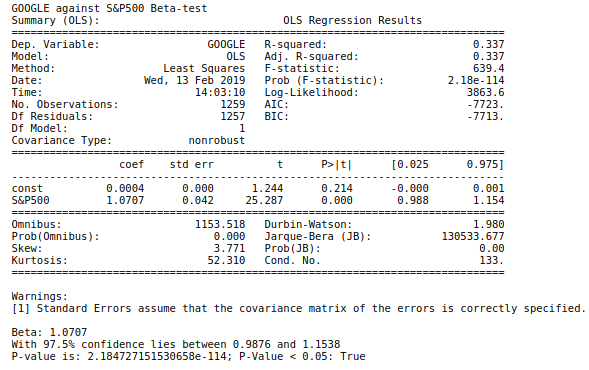
\includegraphics[width=\textwidth]{imgs/beta_1.png}
         \caption{GOOGLE VS S\&P500 Beta-test.}
         \label{fig:beta_1}
     \end{subfigure}
     \hfill
     \begin{subfigure}[b]{0.8\textwidth}
         \centering
         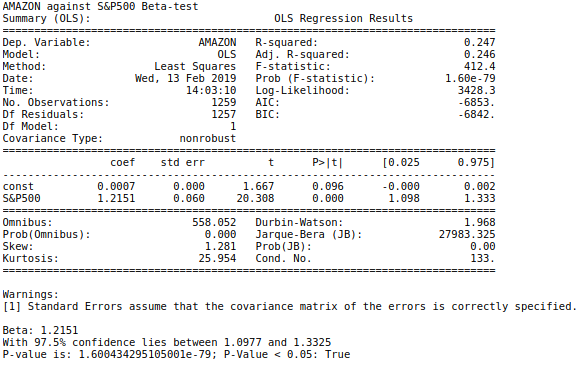
\includegraphics[width=\textwidth]{imgs/beta_2.png}
         \caption{AMAZON vs S\&P500 Beta-test.}
         \label{fig:beta_2}
     \end{subfigure}
\end{figure}

\noindent
The beta-test (Capital Asset Pricing Model (CAPM)) is used to provide a measure which describes the risk/return ratio for the two assets. In this task we use the beta-test to test the relation of a stock price relative to a stock market index (systematic risk). The beta is calculated using Eq.~\ref{eq:beta}. 

\begin{equation} \label{eq:beta}
    Market \ Return = \alpha + (\beta \times stock \ return)
\end{equation}

\noindent
Let’s look at the first result ‘GOOGLE vs S\&P500’ which has a beta of 1.0707 and a p-value which makes this measurement statistically significant. With 95\% confidence that the value lies between 0.9876 and 1.1538. Since the $\beta > 1$, this asset is volatile and moves with the rest of the market. This means that if the market moves in an upwards direction this asset is likely to move in the same direction and the same goes if the market moves in a downward direction. So as a benchmark we know that this asset is positively correlated with the market index as shown in the plot in Fig.~\ref{fig:beta_1_plot}. Looking at the confidence levels, although the beta can be less than 1 it is still a very high value and this means that this stock is likely to move with the market or follows a similar trend. 

\noindent
In the other test ‘AMAZON VS S\&P500’ the beta was 1.2151 and has a p-vale which makes the measurement statistically significant. With 95\% confidence that the value lies between 1.0977 and 1.3325. Like the previous test this stock is volatile and moves with the rest of the market, since it’s correlated according to the test. One must note that the beta confidence levels and the beta is a bit higher than the previous stock which makes this asset to move a bit higher or lower than the benchmark (market-index). This means if the market is moving in an upward direction this stock will see more returns relative to the market and it will see more loses when moving in a downward direction. In fact the beta for the Google stock is close to 1 meaning it will move very similar to the market and this difference between the movements of the two assets can be seen in both the plots Fig.~\ref{fig:beta_1_plot} and Fig.~\ref{fig:beta_2_plot}. 

\begin{figure}[H]
     \centering
     \begin{subfigure}[b]{0.6\textwidth}
         \centering
         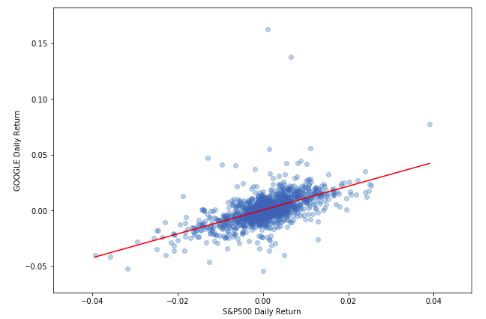
\includegraphics[width=\textwidth]{imgs/beta_1_plot.png}
         \caption{GOOGLE VS S\&P500 Beta-test plot.}
         \label{fig:beta_1_plot}
     \end{subfigure}
     \hfill
     \begin{subfigure}[b]{0.6\textwidth}
         \centering
         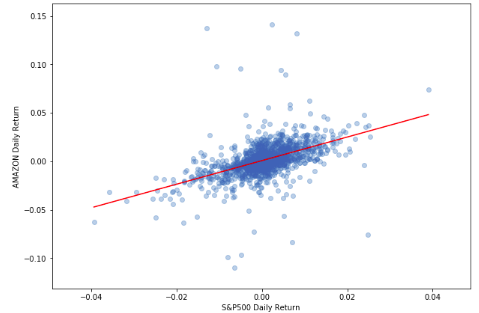
\includegraphics[width=\textwidth]{imgs/beta_2_plot.png}
         \caption{AMAZON vs S\&P500 Beta-test plot.}
         \label{fig:beta_2_plot}
     \end{subfigure}
\end{figure}

\noindent
We would like to add that beta-test does not detect any unsystematic risk. Since we are measuring beta for separate stocks it will give us an indication of how much risk such assets will add or subtract to a portfolio. Such measure does not always predict the stock movements, but it can be a useful indication when building a portfolio as it gives us some indication of how a stock moves with the market. It is also important to note that we used the daily values to measure the beta while it is more common to use the monthly measurements. When using the monthly data, it can faster to compute, easier to identify change in trends and can be good for long term forecasting but if you are looking at daily changes it is better to use daily data. On the other hand, daily is more optimal if you are forecasting for short to medium periods of time but data can be susceptible to noise. Choosing the time period to work with depends on the problem you are trying to solve/predict. 

% END Question (vii) #########################################################################################################
